\documentclass[xcolor={dvipsnames}, aspectratio=169, handout]{beamer}
\usetheme{Darmstadt}
\usecolortheme{dolphin}
\usepackage[logic, complexity, graphs]{commondefns}
\usefonttheme[onlymath]{serif}
\usepackage{csquotes}
\usepackage[style=alphabetic]{biblatex}
\addbibresource{refs.bib}
\usepackage{bussproofs}

\title{Lower Bounds for the Polynomial Calculus\\via the ``Pigeon Dance''}
\author{Imogen Hergeth}
\date{January 2023}
\addtobeamertemplate{navigation symbols}{}{
    \hspace{1em}
    \usebeamerfont{footline}%
    \insertframenumber / \inserttotalframenumber
}


\newcommand{\Sn}{S_n(\KK)}
\newcommand{\Snd}{S_{n, d}(\KK)}
\newcommand{\PHP}{\ensuremath{\neg \mathcal{PHP}^m_n}\xspace}
\newcommand{\Qiij}{Q_{i_1, i_2, j}}
\newcommand{\LT}{\operatorname{LT}}
\newcommand{\Rsem}{R^\mathrm{sem}}
\newcommand{\Rsyn}{R^\mathrm{syn}}
\newcommand{\Dsem}{\Delta^\mathrm{sem}}
\newcommand{\Dsyn}{\Delta^\mathrm{syn}}
\newcommand{\fa}{\text{ for all }}
\renewcommand{\K}{\operatorname{Kill}}
\newcommand{\Is}{{I \setminus \{i_1\}}}
\newcommand{\rhoij}{\rho_{i_1 j_1}}
\newcommand{\xij}{{x_{i_1 j_1}}}

\definecolor{amaranth}{rgb}{0.9, 0.17, 0.31}
\definecolor{pastelred}{rgb}{1.0, 0.41, 0.38}
\definecolor{plum}{rgb}{0.56, 0.27, 0.52}

\definecolor{emerald}{rgb}{0.31, 0.78, 0.47}
\definecolor{caribbeangreen}{rgb}{0.0, 0.8, 0.6}
\definecolor{darkcyan}{rgb}{0.0, 0.55, 0.55}
\definecolor{darkpastelgreen}{rgb}{0.01, 0.75, 0.24}
\definecolor{saffron}{rgb}{0.96, 0.77, 0.19}
\definecolor{chromeyellow}{rgb}{1.0, 0.65, 0.0}
\definecolor{darkorange}{rgb}{1.0, 0.55, 0.0}

\definecolor{bleudefrance}{rgb}{0.19, 0.55, 0.91}

\colorlet{deltaCol}{amaranth}
\colorlet{Rcol}{bleudefrance}
\colorlet{Vcol}{darkorange}

%\includeonlyframes{current}

\begin{document}
\maketitle

\section{Introduction}

\begin{frame}{Overview}
    \tableofcontents[hideallsubsections]
\end{frame}

\subsection{The polynomial calculus}
\begin{frame}{Definition}
    \begin{itemize}[<+->]
        \item Similar to sequent calculus, but lines are polynomials
        \item We use multilinear polynomials $\Sn$\\
            ($xy + xz + v \equiv x^2y + x^3z^5 + v$)
        \item Addition
        \begin{prooftree}
            \AxiomC{$f$}
            \AxiomC{$g$}
            \BinaryInfC{$af + bg$}
        \end{prooftree}
        \item Multiplication
        \begin{prooftree}
            \AxiomC{$f$}
            \UnaryInfC{$f \cdot x$}
        \end{prooftree}
    \end{itemize}
\end{frame}

\begin{frame}{Motivation}
    \begin{itemize}[<+->]
        \item $g$ is provable from $f_1, \ldots, f_n$ if and only if it is in the ideal generated by them
        \item A proof of $g=1$ exists if and only if $f_1, \ldots, f_n$ have no common zeroes
        \item We construct polynomials such that their zeroes correspond to satisfying assignments
        \item Proving $1$ from them is a \textit{refutation}
    \end{itemize}
\end{frame}

\begin{frame}{Example proof}
    \begin{itemize}[<+->]
        \item Try to prove $xy + z$ from $x + 1$ and $z$
    \end{itemize}
    \begin{prooftree}
        \AxiomC{$x+1$}
        \LeftLabel{$(\cdot y)$}
        \UnaryInfC{$xy + y$}
        \AxiomC{$z$}
        \RightLabel{$(+)$}
        \BinaryInfC{$xy + y + z$}
    \end{prooftree}
    \begin{itemize}[<+->]
        \item We now want to subtract $y$
        \item There is no way to prove $y$ from $x+1$ and $z$
        \item Closest to $xy + z$ we can prove is $xy + y + z$
    \end{itemize}
\end{frame}

\begin{frame}{Algebraic view of proofs}
    \begin{itemize}[<+->]
        \item $\textcolor{Vcol}{V}$ are polynomials we can prove \hfill \textcolor{Vcol}{$xy + y + z$}
        \item $\textcolor{deltaCol}{\Delta}$ are leading terms of ones we cannot prove \hfill \textcolor{deltaCol}{$y$}
        \item $\Sn \cong \KK \textcolor{deltaCol}{\Delta} \oplus \textcolor{Vcol}{V}$ \hfill $xy + y + z = -\textcolor{deltaCol}{y} + \textcolor{Vcol}{xy + y + z}$
        \item $\textcolor{Rcol}{R}$ is the projection onto $\textcolor{deltaCol}{\Delta}$ \hfill $\textcolor{Rcol}{R}(xy + y + z) = \textcolor{deltaCol}{y}$
        \item Similarly:\\
        $\textcolor{Vcol}{V_d}, \textcolor{deltaCol}{\Delta_d}, \textcolor{Rcol}{R_d}$ for polynomials up to degree $d$\\
        $\textcolor{Vcol}{V_I}, \textcolor{deltaCol}{\Delta_I}, \textcolor{Rcol}{R_I}$ for polynomials using variables for pigeons in $I$
    \end{itemize}
\end{frame}

\section{The Pigeonhole Principle}
\subsection{Overview}
\begin{frame}{The pigeonhole principle}
    \begin{itemize}[<+->]
        \item If there are $m$ pigeons, $n$ pigeon holes, and $m > n$ then at least two pigeons have to share a hole
        \item Formally: if $m > n$ there is no injection $[m] \tomono [n]$
        \item Variables: $x_{i, j}, i \in [m], n \in [n]$
        \item Assignment of $x_{3, 5}$ corresponds to pigeon $3$ being in hole $5$
    \end{itemize}
    \begin{definition}<+->[\PHP]
        \begin{align*}
            Q_i &\coloneqq 1 - \sum_{j \in [n]} x_{ij} &&\text{for each $i \in [m]$}\\
            \Qiij &\coloneqq x_{i_1j} x_{i_2j} &&\text{for each $i_1 \neq i_2 \in [m], j \in [n]$}
        \end{align*}
    \end{definition}
\end{frame}

\begin{frame}{Main result}
    \begin{theorem}<+->
        For any $m > n$, every polynomial calculus refutation of \PHP must have degree at least $n/2 + 1$.
    \end{theorem}
    \begin{itemize}[<+->]
        \item Characterize $\textcolor{Rcol}{R_d}$ semantically
        \item Problem: only works if $\textcolor{Rcol}{R_I}$ agree on their intersections
        \item Characterize $\textcolor{Rcol}{R_I}$ syntactically
        \item Show the different operators are identical
    \end{itemize}
\end{frame}

\subsection{Valid Pigeon Arrangements}
\begin{frame}{Semantics of \PHP}
    \begin{itemize}[<+->]
        \item What polynomials are derivable from \PHP?
        \item Pigeons cannot share holes
        \item Pigeon assignments are variable assignments
            $$\textcolor{deltaCol}{\Delta}(x) = \begin{cases}
                1, \quad \text{if } x \in \{x_{1, 2}, x_{2, 4}, x_{3, 1}\}\\
                0, \quad \text{otherwise}
            \end{cases}$$
        \item Polynomials are evaluated to $0$ if they allow the assignment
            \begin{align*}
                \textcolor{deltaCol}{\Delta}(1 - x_{1, 1} - x_{1, 2} - x_{1, 3} - x_{1, 4}) &= 0\\
                \textcolor{deltaCol}{\Delta}(x_{1, 1} x_{3, 1}) = \textcolor{deltaCol}{\Delta}(x_{1, 2} x_{2, 2}) &= 0
            \end{align*}
    \end{itemize}
\end{frame}

\begin{frame}{Characterizing $\textcolor{Rcol}{R_I}$}
    \begin{itemize}[<.->]
        \item $M_I$ is the set of all assignments corresponding to injections $I \tomono [m]$
        \item $\textcolor{Vcol}{V_I}$ is polynomials that $M_I$ evaluates to $0$
        \item Define $\textcolor{deltaCol}{\Delta_I}, \textcolor{Rcol}{R_I}$ to be the restrictions of
        $\textcolor{deltaCol}{\Delta}, \textcolor{Rcol}{R}$ onto $I$
        \item Note: this definition completely ignores degrees
    \end{itemize}
\end{frame}

\begin{frame}{Combining $\textcolor{Rcol}{R_I}$}
    \begin{itemize}[<+->]
        \item We want a characterization of $\textcolor{Rcol}{R_d}$, not $\textcolor{Rcol}{R_I}$
        \item $\textcolor{Vcol}{V_d} \coloneqq \bigcup_{|I| \leq d} \textcolor{Vcol}{V_I}$
        \item $\textcolor{Rcol}{R_d} \coloneqq \textcolor{Rcol}{R_{\dom(t)}}(t)$
        \item Does this definition actually work?
        \item Yes it does! But only if $\textcolor{Rcol}{R_I}(t) = \textcolor{Rcol}{R_{\dom(t)}}(t)$ for all $I \supseteq \dom(t)$
    \end{itemize}
\end{frame}

\section{The Pigeon Dance}
\subsection{Characterizing \texorpdfstring{$R_I$}{RI}}
\begin{frame}{Idea}
    \begin{itemize}[<+->]
        \item Goal: define $\textcolor{Rcol}{R_I}(t)$ so that it is independent of $I \setminus \dom(t)$
        \item We first define $\textcolor{deltaCol}{\Delta_I}$ using the pigeon dance
    \end{itemize}
\end{frame}

\newcommand{\pigeon}[3]{
    \node#3 (pigeon#1) at (#2, 1) [label=above right:#1] {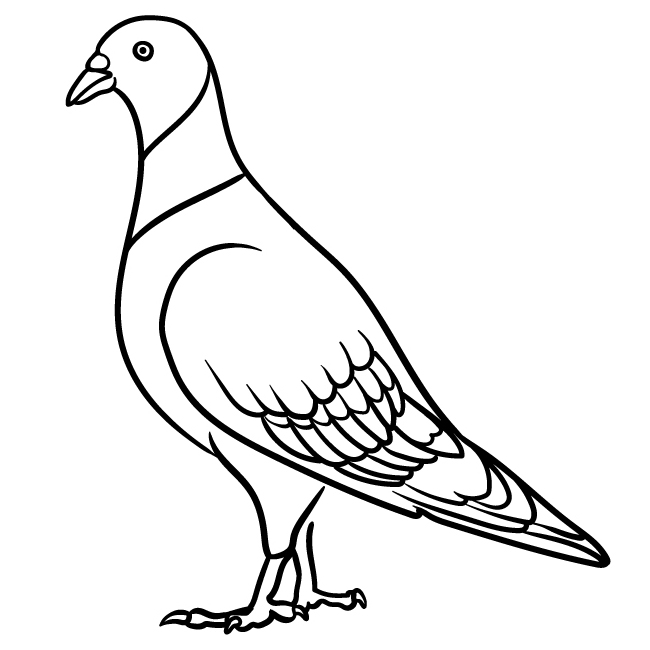
\includegraphics[width=1.5cm]{pigeon.jpg}};
}

\begin{frame}[label=current]{Example}
    \centering

    \begin{tikzpicture}
        \draw[draw=black] (0, 0) rectangle ++(2, 2);
        \draw[draw=black] (2.5, 0) rectangle ++(2, 2);
        \draw[draw=black] (5, 0) rectangle ++(2, 2);
        \draw[draw=black] (7.5, 0) rectangle ++(2, 2);
        \draw[draw=black] (10, 0) rectangle ++(2, 2);

        \pigeon{1}{6}{<+->}
    \end{tikzpicture}
\end{frame}

\begin{frame}{Formalization}
    \begin{itemize}[<+->]
        \item The first pigeon flies to an unoccupied hole to its right
        \item Repeat until all pigeons have moved once
        \item If a pigeon cannot find an empty hole, the dance is aborted
        \item Define $\textcolor{deltaCol}{\Delta_I}$ to be the set of terms that let pigeons complete the dance
        \item $t \in \textcolor{deltaCol}{\Delta_I}$ independent of $I$ since pigeons not in the dance do not affect it
    \end{itemize}
\end{frame}

\begin{frame}{Defining $\textcolor{Rcol}{R_I}$}
    \begin{itemize}[<+->]
        \item We need $\textcolor{Rcol}{R_I}(t) = f$ with $\LT(f) \preceq t$ and $t = f \mod \textcolor{Vcol}{V_I}$
        \item If $t \in \textcolor{deltaCol}{\Delta_I}$, then $f \coloneqq t$
        \item Otherwise, we use $Q_{i_1} = 0$ to derive
            \begin{align*}
                t &= x_{i_1 j_1} \cdots x_{i_d j_d}\\
                &= - \sum_{j' < j_1} x_{i_1 j'} x_{i_2 j_2} \cdots x_{i_d j_d} + x_{i_2 j_2} \cdots x_{i_d j_d} - \sum_{j' > j_1} x_{i_1 j'} x_{i_2 j_2} \cdots x_{i_d j_d} \mod \textcolor{Vcol}{V_I}.
            \end{align*}
        \item The first two summands are $\prec t$ and can be ignored
        \item Any terms with $j' \in \{j_2, \ldots, j_d\}$ are $0$ and can be ignored
    \end{itemize}
\end{frame}

\begin{frame}{Defining $\textcolor{Rcol}{R_I}$ (cont.)}
    \begin{itemize}[<+->]
        \item Remaining terms have $i > i_1$, $j' > j_1$, and $j' \not\in \{j_2, \ldots, j_d\}$
        \item Repeat the same process with all of them
        \item At each step the next $i$ has $x_{i j}$ replaced with $x_{i j'}$ for some unused $j' > j$
        \item This is the pigeon dance!
        \item Since $t \not\in \textcolor{deltaCol}{\Delta_I}$ the dance cannot be completed
        \item Process terminates with $\LT(f) \prec t$ and $t = f \mod \textcolor{Vcol}{V_I}$
    \end{itemize}
\end{frame}

\subsection{Properties of the dance}
\begin{frame}{The $\K$ operator}
    \begin{itemize}[<+->]
        \item Idea: operator that lets us block specific holes
        \item The $\K$ operator kills the first pigeon and moves its hole to the left
        \item $\K(x_{i_1 j_1} \cdots x_{i_d, j_d}) = x_{i_2 j'_2} \cdots x_{i_d j'_d}$ with\\
            $$j'_k \coloneqq \begin{cases}
                    j_k + 1, &\text{if } j_k < j_1\\
                    j_k, &\text{if } j_k > j_1.
                \end{cases}$$
    \end{itemize}
\end{frame}

\begin{frame}{The dance in terms of $\K$}
    \begin{theorem}<.->
        $x_{i_1 j_1} \cdots x_{i_d j_d} \in \textcolor{deltaCol}{\Delta_I}$ if and only if there is a $j' > j_1$ such that
        $\K(x_{i_1 j'} \cdots x_{i_d j_d}) \in \textcolor{deltaCol}{\Delta_I}$.
    \end{theorem}
    \begin{proof}[Proof sketch\nopunct]<+->
        This operator effectively moves the first pigeon to an empty hole to its right and then kills it.
        This is the same as each step in the dance, where the first pigeon flies to some free hole to its right and then occupies it.
    \end{proof}
\end{frame}

\begin{frame}{Closure of $\textcolor{deltaCol}{\Delta_I}$}
     \begin{theorem}<+->
        $\textcolor{deltaCol}{\Delta_I}$ is closed under $\K$.
     \end{theorem}
    \begin{proof}[Proof sketch\nopunct]<+->
        If $t \in \textcolor{deltaCol}{\Delta_I}$ then the pigeons can complete their dance. During this the first pigeon will start at
        $j$ and fly to $j'$. Killing the pigeon frees up $j'$ so any other pigeon that wanted to use $j$ can use it instead.
    \end{proof}
\end{frame}

\begin{frame}{The lower bound}
    \begin{theorem}<+->
        If $|I| \leq (n+1) / 2, t \in \textcolor{deltaCol}{\Delta_I}$ and the minimal element $i$ of $I$ is not in $\dom(t)$, then there exists a $j \in [n]$
        such that $\K(x_{ij} t) \in \textcolor{deltaCol}{\Delta_I}$.
    \end{theorem}
    \begin{proof}[Proof sketch\nopunct{}]<+->
        At most $$
            |\dom(t)| \leq |I \setminus \{i\}| \leq \frac{n - 1}{2}
        $$ pigeons involved in the dance, each occupying two holes. Thus the total number of holes is $n - 1$ and one hole
        $j$ remains free. For the purposes of the dance, $\K(x_{ij} t)$ is the same as $t$ since the only difference is
        $j$ being moved to the left.
    \end{proof}
\end{frame}

\section{Conclusion}

\begin{frame}{Putting things together}
    \begin{itemize}[<+->]
        \item Show that the two operators are identical
        \item Induction over $|I|$ providing an $a \in M_I$ with $a(f) \neq 0$ for any $f \in \KK \textcolor{deltaCol}{\Delta_I}$
        \item Remove variables $x_{ij}$ for minimal $i \in I$ from $f$
        \item Inductive assumption gives us $a' \in M_{I\setminus \{i\}}$ with $a'(f') \neq 0$
        \item Pick a $j$ such that $\K(x_{i j} t) \in \textcolor{deltaCol}{\Delta_I}$
        \item Extend assignment to $I$ with $a(f) \neq 0$
    \end{itemize}
\end{frame}

\begin{frame}{Summary}
    \begin{itemize}[<+->]
        \item If $d \leq n/2 + 1$, then definition of $\textcolor{Rcol}{R_I}$ via the pigeon dance and via $M_I$ are identical
        \item Pigeons not in the dance do not affect its success, so $\textcolor{Rcol}{R_I}(t) = \textcolor{Rcol}{R_{\dom(t)}}(t)$
        \item $\textcolor{Vcol}{V_d}$ is precisely polynomials identically zero on $M_I$
        \item $\textcolor{Rcol}{R_d} \neq 0$
        \item There is no refutation of \PHP with $d \leq n/2 +1$
    \end{itemize}
\end{frame}

\end{document}